\begin{auf}
    364
\end{auf}
Vom gleichen Anfangszustand 1 mit $p_1=1bar$, $V_1=1dm^3$ und $T_1=600K$ ausgehend expandiert ein Gas auf zwei verschiedenen Wegen zum gleichen	Endzustand 2 mit $V_2=2V_1$ und $T_2=\frac{T_1}{2}$. Der Weg 1-3-2 besteht aus einer Isotherme von 1 nach 3 und einer Isochore von 3 nach 2, der Weg 1-4-2 aus einer Isochore von 1 nach 4 und einer Isotherme von 4	nach 2. Wie groß sind auf beiden Wegen jeweils die verrichtete Arbeit $W$, die Änderung der inneren Energie des Gases $\Delta U$ und die ausgetauschte Wärme $Q$? $\kappa=1+\left(\frac{R_S}{c_v}\right)=1.4$.
\begin{figure}[h]
    \centering
    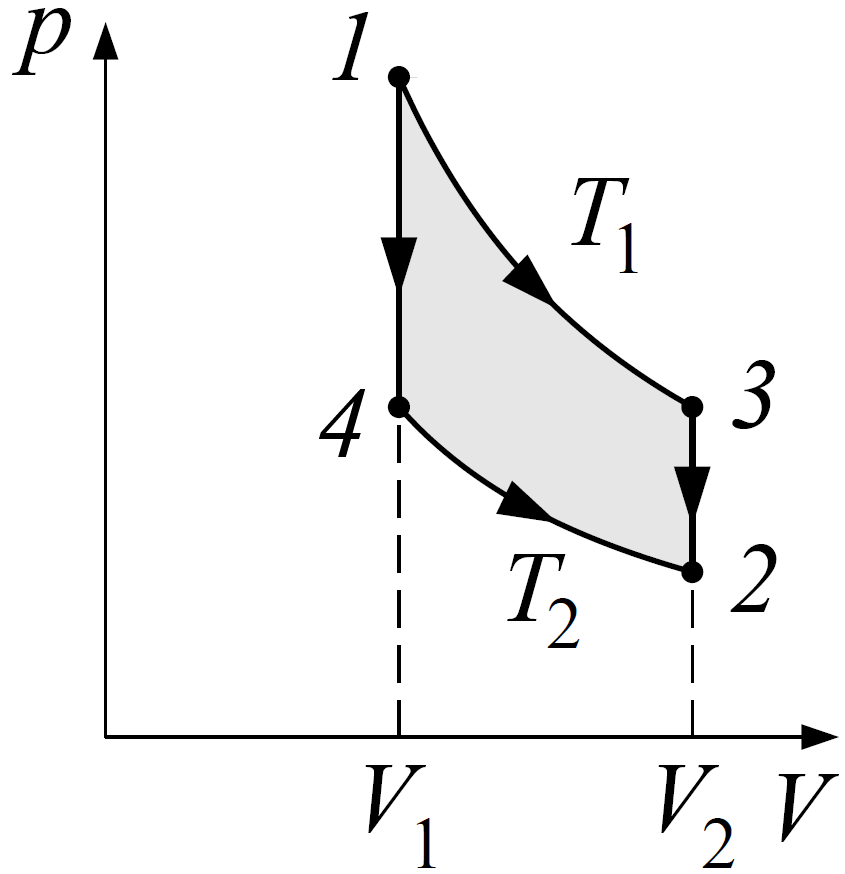
\includegraphics[height=5cm]{images/364_0.png}
    \caption{Versuchsaufbau Aufgabe 364}
\end{figure}